\documentclass{article}
\usepackage{fullpage,color,pgf,tikz}
\usepackage{authblk}
\title{Logic behind the bitsets used for updating diploids in multilocus simulations}
\author[1]{Kevin R. Thornton}
\affil[1]{Department of Ecology and Evolutionary Biology, UC Irvine}
\date{}
\begin{document}
\maketitle
\section*{Intro}
This document is my reminder of the setup and logic behind the code to generate the next generation's diploids in multilocus simulations.
\section*{The setup}

Simulations of multiple partially-linked loci require that we take two parents, recombine their genomes, and then create a new diploid.  In these simulations, parents are represented as vectors of pairs of iterators to gametes.  Each pair is the parent's genotype at a particular locus, and we allow for partial linkage between each locus.  This scheme is cartooned in Figure \ref{concept}.

\begin{figure}[!h]
  \centering
  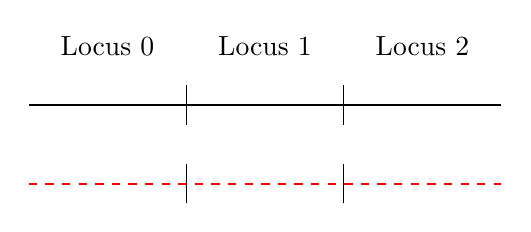
\begin{tikzpicture}
    %locus labels
    \draw (1,2) node[above]{Locus $0$};
    \draw (3,2) node[above]{Locus $1$};
    \draw (5,2) node[above]{Locus $2$};
    % p1g1
    \path[draw,thick](0,1.5) -- (6,1.5);
    \path[draw](2,1.25)--(2,1.75); 
    \path[draw](4,1.25)--(4,1.75);
    
    % p1g2
    \path[draw,color=red,dashed,thick](0,0.5) -- (6,0.5);
    \path[draw](2,0.25)--(2,0.75);  
     \path[draw](4,0.25)--(4,0.75);
  \end{tikzpicture} 
  \caption{\label{concept}Conceptual representation of multiple loci.  Shown is a diploid genotype for 3 loci labeled 0 through 2.  Black and red dashed lines represent alleles for each locus (paternal and maternal, for example).  Vertical lines separate the three loci and we imagine that recombination may happen at these vertical lines at some rate.}
  \end{figure}

It is a trivial matter to generate the recombinant gametes using existing \texttt{fwdpp} routines.  For example, if there is no crossover between the three loci (\textit{e.g.}, the rates at the two vertical bars in Figure \ref{concept} are all zero), then recombination in on parent may lead to a situation like that shown in Figure \ref{simple}.  After the recombination event, we can simply pick either the top or botom ``row'' of scrambled gametes in Figure \ref{simple} with probability $1/2$ each and choose that row to be passed on to the next generation.
  

\begin{figure}[!h]
  \centering
  \begin{tikzpicture}
    % p1g1
    \path[draw,thick](0,1.5) -- (1,1.5);
    \path[draw,color=red,dashed,thick](1,1.5) -- (3,1.5);
    \path[draw,thick](3,1.5) -- (5,1.5);
    \path[draw,color=red,dashed,thick](5,1.5) -- (6,1.5);
    \path[draw](2,1.25)--(2,1.75); 
    \path[draw](4,1.25)--(4,1.75);
    
    % p1g2
    \path[draw,color=red,dashed,thick](0,0.5) -- (1,0.5);
    \path[draw,thick](1,0.5) -- (3,0.5);
    \path[draw,color=red,dashed,thick](3,0.5) -- (5,0.5);
    \path[draw,thick](5,0.5) -- (6,0.5);
    \path[draw](2,0.25)--(2,0.75);  
     \path[draw](4,0.25)--(4,0.75);
  \end{tikzpicture} 
  \caption{\label{simple}Odd number of crossovers within loci 0 and 1.  No crossover between the loci.}
\end{figure}

Things get a little more complex when crossovers within \textit{and} between loci are occurring.  Figure \ref{xo} shows what we want parental gametes to look like after recombination in a more complex case.

\begin{figure}[!h]
  \centering
  \begin{tikzpicture}
    % p1g1
    \path[draw,thick](0,1.5) -- (1,1.5);
    \path[draw,color=red,dashed,thick](1,1.5) -- (2,1.5);
    \path[draw,thick](2,1.5) -- (3,1.5);  
     \path[draw,color=red,dashed,thick](3,1.5) -- (5,1.5);  
     \path[draw,thick](5,1.5) -- (6,1.5); 
     \path[draw](2,1.25)--(2,1.75);  
     \path[draw](4,1.25)--(4,1.75);
    
    % p1g2
    \path[draw,color=red,dashed,thick](0,0.5) -- (1,0.5);
    \path[draw,thick](1,0.5) -- (2,0.5); 
    \path[draw,thick,color=red,dashed](2,0.5) -- (3,0.5);  
     \path[draw,thick](3,0.5) -- (5,0.5);  
     \path[draw,color=red,dashed,thick](5,0.5) -- (6,0.5); 
     \path[draw](2,0.25)--(2,0.75);  
     \path[draw](4,0.25)--(4,0.75);
  \end{tikzpicture} 
  \caption{\label{xo}Odd number of crossovers within loci 0 and 1.  Crossover between 0 and 1.}
\end{figure}

The question is how to generate outcomes like Figure \ref{xo} efficiently.
\section*{The solution}
\end{document}
